\documentclass[12pt]{article}
\usepackage{tikz}
\usepackage{amsmath}
% Underlining package
\usepackage{ulem}
\usetikzlibrary{calc}
\usetikzlibrary{angles,quotes}
\usepackage[a4paper, portrait, margin=1cm]{geometry}
\usepackage{fancyhdr}

\newcommand{\HeadingQuestions}{%
\section*{\Large Name: \underline{\hspace{8cm}} \hfill Date: \underline{\hspace{3cm}}}%
\vspace{-3mm}\par
\textbf{Volume rectangular prisms}\vspace{1pt}\hrule
}

% raise footer with page number; no header
\fancypagestyle{myfancypagestyle}{
  \fancyhf{}% clear all header and footer fields
  \renewcommand{\headrulewidth}{0pt} % no rule under header
  \fancyfoot[C] {\thepage} \setlength{\footskip}{14.5pt} % raise page number allowed min 14.5pt
}
\pagestyle{myfancypagestyle}  % apply myfancypagestyle

\newcounter{minipagecount}

\begin{document}
\HeadingQuestions
\vspace{8mm}

\begin{minipage}{0.50\textwidth}
  \refstepcounter{minipagecount}
  \noindent{(\theminipagecount)}\quad
  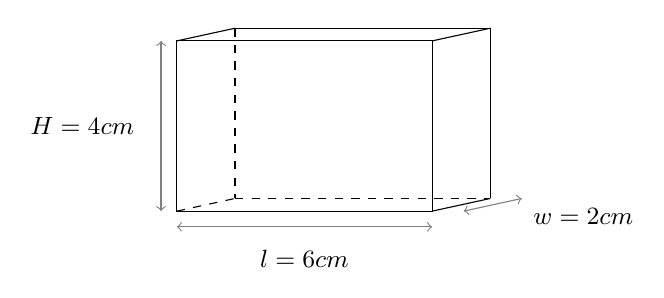
\begin{tikzpicture}[scale=1.0, baseline=(current bounding box.north)]
     \begin{scope}[rotate=0]

    % front face
    \coordinate (E) at (0,0);
    \coordinate (F) at (3.243,0);
    \coordinate (G) at (3.243,2.162);
    \coordinate (H) at (0,2.162);

    % back face skew shift
    \coordinate (K) at ($(E)+(0.739, 0.161)$);
    \coordinate (L) at ($(F)+(0.739, 0.161)$);
    \coordinate (M) at ($(G)+(0.739, 0.161)$);
    \coordinate (N) at ($(H)+(0.739, 0.161)$);

    % draw prism edges
    \draw[] (E)--(F)--(G)--(H)--cycle;
    \draw[dashed] (E)--(K);
    \draw[] (F)--(L);
    \draw[] (G)--(M);
    \draw[] (H)--(N);
    \draw[dashed] (K)--(L);
    \draw[] (L)--(M);
    \draw[] (M)--(N);
    \draw[dashed] (N)--(K);

    % label corners
    % \node[above left] at (E) {E};
    % \node[below right] at (F) {F};
    % \node[above right] at (G) {G};
    % \node[above left] at (H) {H};
    % \node[below left] at (K) {K};
    % \node[below right] at (L) {L};
    % \node[above right] at (M) {M};
    % \node[above left] at (N) {N};

    % dimension lines enabled
    \coordinate (P1offAB) at ($ (E)+(0,-0.2) $);
    \coordinate (P2offAB) at ($ (F)+(0,-0.2) $);
    \draw[<->,gray] (P1offAB)--(P2offAB);
    \node[black, fill=white, fill opacity=1.0, text opacity=1, inner sep=1pt]
        at ($ (P1offAB)!0.5!(P2offAB) + (0,-0.4) $) {\small $l=6 cm$};

    \coordinate (P1offAD) at ($ (E)+(-0.2,0) $);
    \coordinate (P2offAD) at ($ (H)+(-0.2,0) $);
    \draw[<->,gray] (P1offAD)--(P2offAD);
    \node[black, fill=white, fill opacity=1.0, text opacity=1, inner sep=1pt]
        at ($ (P1offAD)!0.5!(P2offAD) + (-1.0,0) $) {\small $H=4 cm$};

    \coordinate (P1offBF) at ($ (F)+(0.4,0) $);
    \coordinate (P2offBF) at ($ (L)+(0.4,0) $);
    \draw[<->,gray] (P1offBF)--(P2offBF);
    \node[black, fill=white, fill opacity=1.0, text opacity=1, inner sep=1pt]
        at ($ (P1offBF)!0.5!(P2offBF) + (1.15,-0.15) $) {\small $w=2 cm$};
    \end{scope}
\end{tikzpicture}
\end{minipage}
\hfill
\begin{minipage}{.5\textwidth}
  \begin{align*}
  \text{Volume} &= lwH \\
  \text{Volume} &= \dotuline{~~~~~} \,\text{cm} \times \dotuline{~~~~~} \,\text{cm} \times \dotuline{~~~~~} \,\text{cm} \\
  \text{Volume} &= \dotuline{~~~~~} \,\text{cm}^3
  \end{align*}
\end{minipage}
\par\vspace{1cm}\begin{minipage}{0.50\textwidth}
  \refstepcounter{minipagecount}
  \noindent{(\theminipagecount)}\quad
  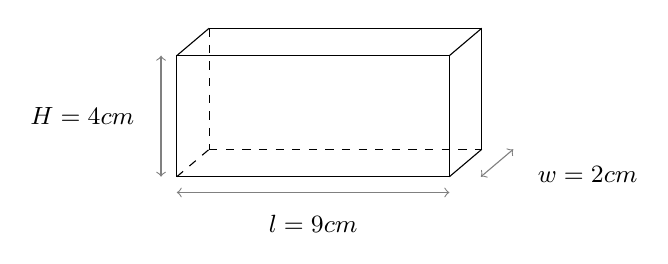
\begin{tikzpicture}[scale=1.0, baseline=(current bounding box.north)]
     \begin{scope}[rotate=0]

    % front face
    \coordinate (E) at (0,0);
    \coordinate (F) at (3.462,0);
    \coordinate (G) at (3.462,1.538);
    \coordinate (H) at (0,1.538);

    % back face skew shift
    \coordinate (K) at ($(E)+(0.411, 0.348)$);
    \coordinate (L) at ($(F)+(0.411, 0.348)$);
    \coordinate (M) at ($(G)+(0.411, 0.348)$);
    \coordinate (N) at ($(H)+(0.411, 0.348)$);

    % draw prism edges
    \draw[] (E)--(F)--(G)--(H)--cycle;
    \draw[dashed] (E)--(K);
    \draw[] (F)--(L);
    \draw[] (G)--(M);
    \draw[] (H)--(N);
    \draw[dashed] (K)--(L);
    \draw[] (L)--(M);
    \draw[] (M)--(N);
    \draw[dashed] (N)--(K);

    % label corners
    % \node[above left] at (E) {E};
    % \node[below right] at (F) {F};
    % \node[above right] at (G) {G};
    % \node[above left] at (H) {H};
    % \node[below left] at (K) {K};
    % \node[below right] at (L) {L};
    % \node[above right] at (M) {M};
    % \node[above left] at (N) {N};

    % dimension lines enabled
    \coordinate (P1offAB) at ($ (E)+(0,-0.2) $);
    \coordinate (P2offAB) at ($ (F)+(0,-0.2) $);
    \draw[<->,gray] (P1offAB)--(P2offAB);
    \node[black, fill=white, fill opacity=1.0, text opacity=1, inner sep=1pt]
        at ($ (P1offAB)!0.5!(P2offAB) + (0,-0.4) $) {\small $l=9 cm$};

    \coordinate (P1offAD) at ($ (E)+(-0.2,0) $);
    \coordinate (P2offAD) at ($ (H)+(-0.2,0) $);
    \draw[<->,gray] (P1offAD)--(P2offAD);
    \node[black, fill=white, fill opacity=1.0, text opacity=1, inner sep=1pt]
        at ($ (P1offAD)!0.5!(P2offAD) + (-1.0,0) $) {\small $H=4 cm$};

    \coordinate (P1offBF) at ($ (F)+(0.4,0) $);
    \coordinate (P2offBF) at ($ (L)+(0.4,0) $);
    \draw[<->,gray] (P1offBF)--(P2offBF);
    \node[black, fill=white, fill opacity=1.0, text opacity=1, inner sep=1pt]
        at ($ (P1offBF)!0.5!(P2offBF) + (1.15,-0.15) $) {\small $w=2 cm$};
    \end{scope}
\end{tikzpicture}
\end{minipage}
\hfill
\begin{minipage}{.5\textwidth}
  \begin{align*}
  \text{Volume} &= lwH \\
  \text{Volume} &= \dotuline{~~~~~} \,\text{cm} \times \dotuline{~~~~~} \,\text{cm} \times \dotuline{~~~~~} \,\text{cm} \\
  \text{Volume} &= \dotuline{~~~~~} \,\text{cm}^3
  \end{align*}
\end{minipage}
\par\vspace{1cm}\begin{minipage}{0.50\textwidth}
  \refstepcounter{minipagecount}
  \noindent{(\theminipagecount)}\quad
  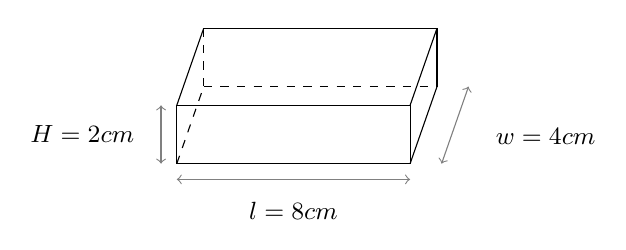
\begin{tikzpicture}[scale=1.0, baseline=(current bounding box.north)]
     \begin{scope}[rotate=0]

    % front face
    \coordinate (E) at (0,0);
    \coordinate (F) at (2.963,0);
    \coordinate (G) at (2.963,0.741);
    \coordinate (H) at (0,0.741);

    % back face skew shift
    \coordinate (K) at ($(E)+(0.342, 0.979)$);
    \coordinate (L) at ($(F)+(0.342, 0.979)$);
    \coordinate (M) at ($(G)+(0.342, 0.979)$);
    \coordinate (N) at ($(H)+(0.342, 0.979)$);

    % draw prism edges
    \draw[] (E)--(F)--(G)--(H)--cycle;
    \draw[dashed] (E)--(K);
    \draw[] (F)--(L);
    \draw[] (G)--(M);
    \draw[] (H)--(N);
    \draw[dashed] (K)--(L);
    \draw[] (L)--(M);
    \draw[] (M)--(N);
    \draw[dashed] (N)--(K);

    % label corners
    % \node[above left] at (E) {E};
    % \node[below right] at (F) {F};
    % \node[above right] at (G) {G};
    % \node[above left] at (H) {H};
    % \node[below left] at (K) {K};
    % \node[below right] at (L) {L};
    % \node[above right] at (M) {M};
    % \node[above left] at (N) {N};

    % dimension lines enabled
    \coordinate (P1offAB) at ($ (E)+(0,-0.2) $);
    \coordinate (P2offAB) at ($ (F)+(0,-0.2) $);
    \draw[<->,gray] (P1offAB)--(P2offAB);
    \node[black, fill=white, fill opacity=1.0, text opacity=1, inner sep=1pt]
        at ($ (P1offAB)!0.5!(P2offAB) + (0,-0.4) $) {\small $l=8 cm$};

    \coordinate (P1offAD) at ($ (E)+(-0.2,0) $);
    \coordinate (P2offAD) at ($ (H)+(-0.2,0) $);
    \draw[<->,gray] (P1offAD)--(P2offAD);
    \node[black, fill=white, fill opacity=1.0, text opacity=1, inner sep=1pt]
        at ($ (P1offAD)!0.5!(P2offAD) + (-1.0,0) $) {\small $H=2 cm$};

    \coordinate (P1offBF) at ($ (F)+(0.4,0) $);
    \coordinate (P2offBF) at ($ (L)+(0.4,0) $);
    \draw[<->,gray] (P1offBF)--(P2offBF);
    \node[black, fill=white, fill opacity=1.0, text opacity=1, inner sep=1pt]
        at ($ (P1offBF)!0.5!(P2offBF) + (1.15,-0.15) $) {\small $w=4 cm$};
    \end{scope}
\end{tikzpicture}
\end{minipage}
\hfill
\begin{minipage}{.5\textwidth}
  \begin{align*}
  \text{Volume} &= lwH \\
  \text{Volume} &= \dotuline{~~~~~} \,\text{cm} \times \dotuline{~~~~~} \,\text{cm} \times \dotuline{~~~~~} \,\text{cm} \\
  \text{Volume} &= \dotuline{~~~~~} \,\text{cm}^3
  \end{align*}
\end{minipage}
\par\vspace{1cm}\begin{minipage}{0.50\textwidth}
  \refstepcounter{minipagecount}
  \noindent{(\theminipagecount)}\quad
  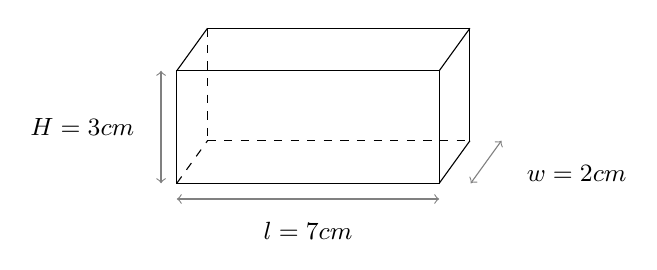
\begin{tikzpicture}[scale=1.0, baseline=(current bounding box.north)]
     \begin{scope}[rotate=0]

    % front face
    \coordinate (E) at (0,0);
    \coordinate (F) at (3.333,0);
    \coordinate (G) at (3.333,1.429);
    \coordinate (H) at (0,1.429);

    % back face skew shift
    \coordinate (K) at ($(E)+(0.39, 0.54)$);
    \coordinate (L) at ($(F)+(0.39, 0.54)$);
    \coordinate (M) at ($(G)+(0.39, 0.54)$);
    \coordinate (N) at ($(H)+(0.39, 0.54)$);

    % draw prism edges
    \draw[] (E)--(F)--(G)--(H)--cycle;
    \draw[dashed] (E)--(K);
    \draw[] (F)--(L);
    \draw[] (G)--(M);
    \draw[] (H)--(N);
    \draw[dashed] (K)--(L);
    \draw[] (L)--(M);
    \draw[] (M)--(N);
    \draw[dashed] (N)--(K);

    % label corners
    % \node[above left] at (E) {E};
    % \node[below right] at (F) {F};
    % \node[above right] at (G) {G};
    % \node[above left] at (H) {H};
    % \node[below left] at (K) {K};
    % \node[below right] at (L) {L};
    % \node[above right] at (M) {M};
    % \node[above left] at (N) {N};

    % dimension lines enabled
    \coordinate (P1offAB) at ($ (E)+(0,-0.2) $);
    \coordinate (P2offAB) at ($ (F)+(0,-0.2) $);
    \draw[<->,gray] (P1offAB)--(P2offAB);
    \node[black, fill=white, fill opacity=1.0, text opacity=1, inner sep=1pt]
        at ($ (P1offAB)!0.5!(P2offAB) + (0,-0.4) $) {\small $l=7 cm$};

    \coordinate (P1offAD) at ($ (E)+(-0.2,0) $);
    \coordinate (P2offAD) at ($ (H)+(-0.2,0) $);
    \draw[<->,gray] (P1offAD)--(P2offAD);
    \node[black, fill=white, fill opacity=1.0, text opacity=1, inner sep=1pt]
        at ($ (P1offAD)!0.5!(P2offAD) + (-1.0,0) $) {\small $H=3 cm$};

    \coordinate (P1offBF) at ($ (F)+(0.4,0) $);
    \coordinate (P2offBF) at ($ (L)+(0.4,0) $);
    \draw[<->,gray] (P1offBF)--(P2offBF);
    \node[black, fill=white, fill opacity=1.0, text opacity=1, inner sep=1pt]
        at ($ (P1offBF)!0.5!(P2offBF) + (1.15,-0.15) $) {\small $w=2 cm$};
    \end{scope}
\end{tikzpicture}
\end{minipage}
\hfill
\begin{minipage}{.5\textwidth}
  \begin{align*}
  \text{Volume} &= lwH \\
  \text{Volume} &= \dotuline{~~~~~} \,\text{cm} \times \dotuline{~~~~~} \,\text{cm} \times \dotuline{~~~~~} \,\text{cm} \\
  \text{Volume} &= \dotuline{~~~~~} \,\text{cm}^3
  \end{align*}
\end{minipage}
\par\vspace{1cm}\begin{minipage}{0.50\textwidth}
  \refstepcounter{minipagecount}
  \noindent{(\theminipagecount)}\quad
  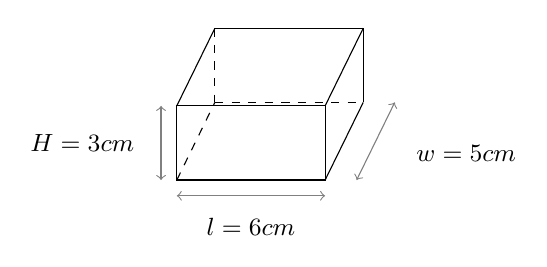
\begin{tikzpicture}[scale=1.0, baseline=(current bounding box.north)]
     \begin{scope}[rotate=0]

    % front face
    \coordinate (Q) at (0,0);
    \coordinate (R) at (1.884,0);
    \coordinate (S) at (1.884,0.942);
    \coordinate (T) at (0,0.942);

    % back face skew shift
    \coordinate (W) at ($(Q)+(0.484, 0.986)$);
    \coordinate (X) at ($(R)+(0.484, 0.986)$);
    \coordinate (Y) at ($(S)+(0.484, 0.986)$);
    \coordinate (Z) at ($(T)+(0.484, 0.986)$);

    % draw prism edges
    \draw[] (Q)--(R)--(S)--(T)--cycle;
    \draw[dashed] (Q)--(W);
    \draw[] (R)--(X);
    \draw[] (S)--(Y);
    \draw[] (T)--(Z);
    \draw[dashed] (W)--(X);
    \draw[] (X)--(Y);
    \draw[] (Y)--(Z);
    \draw[dashed] (Z)--(W);

    % label corners
    % \node[above left] at (Q) {Q};
    % \node[below right] at (R) {R};
    % \node[above right] at (S) {S};
    % \node[above left] at (T) {T};
    % \node[below left] at (W) {W};
    % \node[below right] at (X) {X};
    % \node[above right] at (Y) {Y};
    % \node[above left] at (Z) {Z};

    % dimension lines enabled
    \coordinate (P1offAB) at ($ (Q)+(0,-0.2) $);
    \coordinate (P2offAB) at ($ (R)+(0,-0.2) $);
    \draw[<->,gray] (P1offAB)--(P2offAB);
    \node[black, fill=white, fill opacity=1.0, text opacity=1, inner sep=1pt]
        at ($ (P1offAB)!0.5!(P2offAB) + (0,-0.4) $) {\small $l=6 cm$};

    \coordinate (P1offAD) at ($ (Q)+(-0.2,0) $);
    \coordinate (P2offAD) at ($ (T)+(-0.2,0) $);
    \draw[<->,gray] (P1offAD)--(P2offAD);
    \node[black, fill=white, fill opacity=1.0, text opacity=1, inner sep=1pt]
        at ($ (P1offAD)!0.5!(P2offAD) + (-1.0,0) $) {\small $H=3 cm$};

    \coordinate (P1offBF) at ($ (R)+(0.4,0) $);
    \coordinate (P2offBF) at ($ (X)+(0.4,0) $);
    \draw[<->,gray] (P1offBF)--(P2offBF);
    \node[black, fill=white, fill opacity=1.0, text opacity=1, inner sep=1pt]
        at ($ (P1offBF)!0.5!(P2offBF) + (1.15,-0.15) $) {\small $w=5 cm$};
    \end{scope}
\end{tikzpicture}
\end{minipage}
\hfill
\begin{minipage}{.5\textwidth}
  \begin{align*}
  \text{Volume} &= lwH \\
  \text{Volume} &= \dotuline{~~~~~} \,\text{cm} \times \dotuline{~~~~~} \,\text{cm} \times \dotuline{~~~~~} \,\text{cm} \\
  \text{Volume} &= \dotuline{~~~~~} \,\text{cm}^3
  \end{align*}
\end{minipage}
\par\vspace{1cm}\begin{minipage}{0.50\textwidth}
  \refstepcounter{minipagecount}
  \noindent{(\theminipagecount)}\quad
  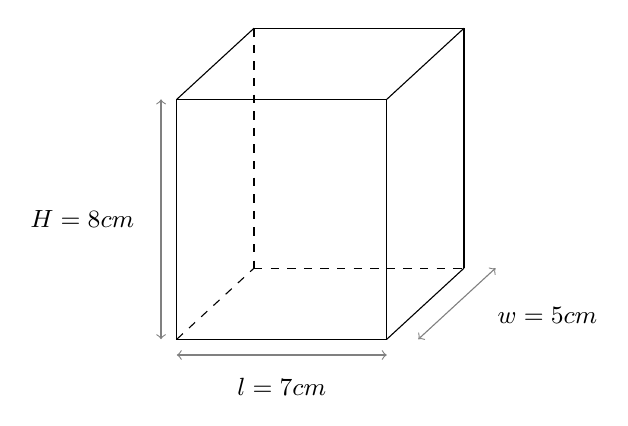
\begin{tikzpicture}[scale=1.0, baseline=(current bounding box.north)]
     \begin{scope}[rotate=0]

    % front face
    \coordinate (E) at (0,0);
    \coordinate (F) at (2.667,0);
    \coordinate (G) at (2.667,3.047);
    \coordinate (H) at (0,3.047);

    % back face skew shift
    \coordinate (K) at ($(E)+(0.981, 0.903)$);
    \coordinate (L) at ($(F)+(0.981, 0.903)$);
    \coordinate (M) at ($(G)+(0.981, 0.903)$);
    \coordinate (N) at ($(H)+(0.981, 0.903)$);

    % draw prism edges
    \draw[] (E)--(F)--(G)--(H)--cycle;
    \draw[dashed] (E)--(K);
    \draw[] (F)--(L);
    \draw[] (G)--(M);
    \draw[] (H)--(N);
    \draw[dashed] (K)--(L);
    \draw[] (L)--(M);
    \draw[] (M)--(N);
    \draw[dashed] (N)--(K);

    % label corners
    % \node[above left] at (E) {E};
    % \node[below right] at (F) {F};
    % \node[above right] at (G) {G};
    % \node[above left] at (H) {H};
    % \node[below left] at (K) {K};
    % \node[below right] at (L) {L};
    % \node[above right] at (M) {M};
    % \node[above left] at (N) {N};

    % dimension lines enabled
    \coordinate (P1offAB) at ($ (E)+(0,-0.2) $);
    \coordinate (P2offAB) at ($ (F)+(0,-0.2) $);
    \draw[<->,gray] (P1offAB)--(P2offAB);
    \node[black, fill=white, fill opacity=1.0, text opacity=1, inner sep=1pt]
        at ($ (P1offAB)!0.5!(P2offAB) + (0,-0.4) $) {\small $l=7 cm$};

    \coordinate (P1offAD) at ($ (E)+(-0.2,0) $);
    \coordinate (P2offAD) at ($ (H)+(-0.2,0) $);
    \draw[<->,gray] (P1offAD)--(P2offAD);
    \node[black, fill=white, fill opacity=1.0, text opacity=1, inner sep=1pt]
        at ($ (P1offAD)!0.5!(P2offAD) + (-1.0,0) $) {\small $H=8 cm$};

    \coordinate (P1offBF) at ($ (F)+(0.4,0) $);
    \coordinate (P2offBF) at ($ (L)+(0.4,0) $);
    \draw[<->,gray] (P1offBF)--(P2offBF);
    \node[black, fill=white, fill opacity=1.0, text opacity=1, inner sep=1pt]
        at ($ (P1offBF)!0.5!(P2offBF) + (1.15,-0.15) $) {\small $w=5 cm$};
    \end{scope}
\end{tikzpicture}
\end{minipage}
\hfill
\begin{minipage}{.5\textwidth}
  \begin{align*}
  \text{Volume} &= lwH \\
  \text{Volume} &= \dotuline{~~~~~} \,\text{cm} \times \dotuline{~~~~~} \,\text{cm} \times \dotuline{~~~~~} \,\text{cm} \\
  \text{Volume} &= \dotuline{~~~~~} \,\text{cm}^3
  \end{align*}
\end{minipage}
\par\vspace{1cm}\begin{minipage}{0.50\textwidth}
  \refstepcounter{minipagecount}
  \noindent{(\theminipagecount)}\quad
  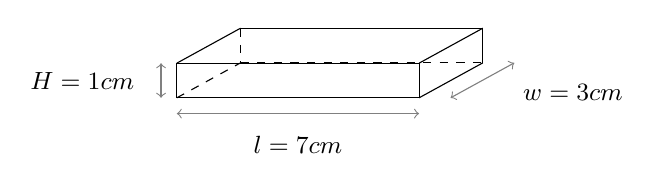
\begin{tikzpicture}[scale=1.0, baseline=(current bounding box.north)]
     \begin{scope}[rotate=0]

    % front face
    \coordinate (A) at (0,0);
    \coordinate (B) at (3.077,0);
    \coordinate (C) at (3.077,0.44);
    \coordinate (D) at (0,0.44);

    % back face skew shift
    \coordinate (E) at ($(A)+(0.809, 0.444)$);
    \coordinate (F) at ($(B)+(0.809, 0.444)$);
    \coordinate (G) at ($(C)+(0.809, 0.444)$);
    \coordinate (H) at ($(D)+(0.809, 0.444)$);

    % draw prism edges
    \draw[] (A)--(B)--(C)--(D)--cycle;
    \draw[dashed] (A)--(E);
    \draw[] (B)--(F);
    \draw[] (C)--(G);
    \draw[] (D)--(H);
    \draw[dashed] (E)--(F);
    \draw[] (F)--(G);
    \draw[] (G)--(H);
    \draw[dashed] (H)--(E);

    % label corners
    % \node[above left] at (A) {A};
    % \node[below right] at (B) {B};
    % \node[above right] at (C) {C};
    % \node[above left] at (D) {D};
    % \node[below left] at (E) {E};
    % \node[below right] at (F) {F};
    % \node[above right] at (G) {G};
    % \node[above left] at (H) {H};

    % dimension lines enabled
    \coordinate (P1offAB) at ($ (A)+(0,-0.2) $);
    \coordinate (P2offAB) at ($ (B)+(0,-0.2) $);
    \draw[<->,gray] (P1offAB)--(P2offAB);
    \node[black, fill=white, fill opacity=1.0, text opacity=1, inner sep=1pt]
        at ($ (P1offAB)!0.5!(P2offAB) + (0,-0.4) $) {\small $l=7 cm$};

    \coordinate (P1offAD) at ($ (A)+(-0.2,0) $);
    \coordinate (P2offAD) at ($ (D)+(-0.2,0) $);
    \draw[<->,gray] (P1offAD)--(P2offAD);
    \node[black, fill=white, fill opacity=1.0, text opacity=1, inner sep=1pt]
        at ($ (P1offAD)!0.5!(P2offAD) + (-1.0,0) $) {\small $H=1 cm$};

    \coordinate (P1offBF) at ($ (B)+(0.4,0) $);
    \coordinate (P2offBF) at ($ (F)+(0.4,0) $);
    \draw[<->,gray] (P1offBF)--(P2offBF);
    \node[black, fill=white, fill opacity=1.0, text opacity=1, inner sep=1pt]
        at ($ (P1offBF)!0.5!(P2offBF) + (1.15,-0.15) $) {\small $w=3 cm$};
    \end{scope}
\end{tikzpicture}
\end{minipage}
\hfill
\begin{minipage}{.5\textwidth}
  \begin{align*}
  \text{Volume} &= lwH \\
  \text{Volume} &= \dotuline{~~~~~} \,\text{cm} \times \dotuline{~~~~~} \,\text{cm} \times \dotuline{~~~~~} \,\text{cm} \\
  \text{Volume} &= \dotuline{~~~~~} \,\text{cm}^3
  \end{align*}
\end{minipage}
\par\vspace{1cm}\begin{minipage}{0.50\textwidth}
  \refstepcounter{minipagecount}
  \noindent{(\theminipagecount)}\quad
  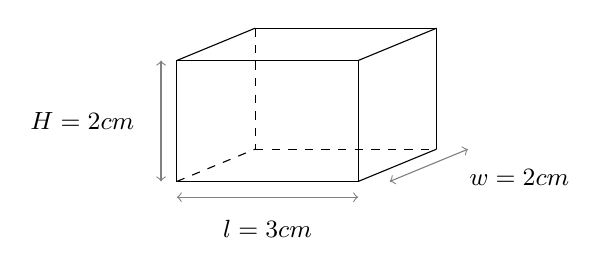
\begin{tikzpicture}[scale=1.0, baseline=(current bounding box.north)]
     \begin{scope}[rotate=0]

    % front face
    \coordinate (K) at (0,0);
    \coordinate (L) at (2.304,0);
    \coordinate (M) at (2.304,1.536);
    \coordinate (N) at (0,1.536);

    % back face skew shift
    \coordinate (Q) at ($(K)+(0.994, 0.41)$);
    \coordinate (R) at ($(L)+(0.994, 0.41)$);
    \coordinate (S) at ($(M)+(0.994, 0.41)$);
    \coordinate (T) at ($(N)+(0.994, 0.41)$);

    % draw prism edges
    \draw[] (K)--(L)--(M)--(N)--cycle;
    \draw[dashed] (K)--(Q);
    \draw[] (L)--(R);
    \draw[] (M)--(S);
    \draw[] (N)--(T);
    \draw[dashed] (Q)--(R);
    \draw[] (R)--(S);
    \draw[] (S)--(T);
    \draw[dashed] (T)--(Q);

    % label corners
    % \node[above left] at (K) {K};
    % \node[below right] at (L) {L};
    % \node[above right] at (M) {M};
    % \node[above left] at (N) {N};
    % \node[below left] at (Q) {Q};
    % \node[below right] at (R) {R};
    % \node[above right] at (S) {S};
    % \node[above left] at (T) {T};

    % dimension lines enabled
    \coordinate (P1offAB) at ($ (K)+(0,-0.2) $);
    \coordinate (P2offAB) at ($ (L)+(0,-0.2) $);
    \draw[<->,gray] (P1offAB)--(P2offAB);
    \node[black, fill=white, fill opacity=1.0, text opacity=1, inner sep=1pt]
        at ($ (P1offAB)!0.5!(P2offAB) + (0,-0.4) $) {\small $l=3 cm$};

    \coordinate (P1offAD) at ($ (K)+(-0.2,0) $);
    \coordinate (P2offAD) at ($ (N)+(-0.2,0) $);
    \draw[<->,gray] (P1offAD)--(P2offAD);
    \node[black, fill=white, fill opacity=1.0, text opacity=1, inner sep=1pt]
        at ($ (P1offAD)!0.5!(P2offAD) + (-1.0,0) $) {\small $H=2 cm$};

    \coordinate (P1offBF) at ($ (L)+(0.4,0) $);
    \coordinate (P2offBF) at ($ (R)+(0.4,0) $);
    \draw[<->,gray] (P1offBF)--(P2offBF);
    \node[black, fill=white, fill opacity=1.0, text opacity=1, inner sep=1pt]
        at ($ (P1offBF)!0.5!(P2offBF) + (1.15,-0.15) $) {\small $w=2 cm$};
    \end{scope}
\end{tikzpicture}
\end{minipage}
\hfill
\begin{minipage}{.5\textwidth}
  \begin{align*}
  \text{Volume} &= lwH \\
  \text{Volume} &= \dotuline{~~~~~} \,\text{cm} \times \dotuline{~~~~~} \,\text{cm} \times \dotuline{~~~~~} \,\text{cm} \\
  \text{Volume} &= \dotuline{~~~~~} \,\text{cm}^3
  \end{align*}
\end{minipage}
\par\vspace{1cm}\begin{minipage}{0.50\textwidth}
  \refstepcounter{minipagecount}
  \noindent{(\theminipagecount)}\quad
  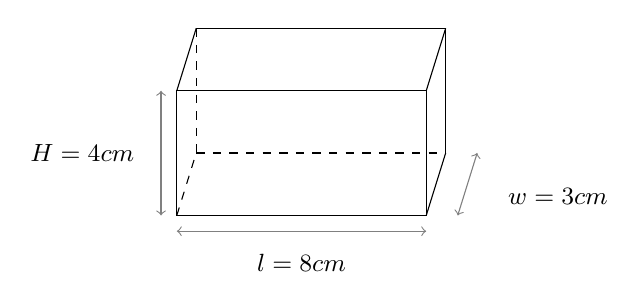
\begin{tikzpicture}[scale=1.0, baseline=(current bounding box.north)]
     \begin{scope}[rotate=0]

    % front face
    \coordinate (Q) at (0,0);
    \coordinate (R) at (3.168,0);
    \coordinate (S) at (3.168,1.584);
    \coordinate (T) at (0,1.584);

    % back face skew shift
    \coordinate (W) at ($(Q)+(0.247, 0.794)$);
    \coordinate (X) at ($(R)+(0.247, 0.794)$);
    \coordinate (Y) at ($(S)+(0.247, 0.794)$);
    \coordinate (Z) at ($(T)+(0.247, 0.794)$);

    % draw prism edges
    \draw[] (Q)--(R)--(S)--(T)--cycle;
    \draw[dashed] (Q)--(W);
    \draw[] (R)--(X);
    \draw[] (S)--(Y);
    \draw[] (T)--(Z);
    \draw[dashed] (W)--(X);
    \draw[] (X)--(Y);
    \draw[] (Y)--(Z);
    \draw[dashed] (Z)--(W);

    % label corners
    % \node[above left] at (Q) {Q};
    % \node[below right] at (R) {R};
    % \node[above right] at (S) {S};
    % \node[above left] at (T) {T};
    % \node[below left] at (W) {W};
    % \node[below right] at (X) {X};
    % \node[above right] at (Y) {Y};
    % \node[above left] at (Z) {Z};

    % dimension lines enabled
    \coordinate (P1offAB) at ($ (Q)+(0,-0.2) $);
    \coordinate (P2offAB) at ($ (R)+(0,-0.2) $);
    \draw[<->,gray] (P1offAB)--(P2offAB);
    \node[black, fill=white, fill opacity=1.0, text opacity=1, inner sep=1pt]
        at ($ (P1offAB)!0.5!(P2offAB) + (0,-0.4) $) {\small $l=8 cm$};

    \coordinate (P1offAD) at ($ (Q)+(-0.2,0) $);
    \coordinate (P2offAD) at ($ (T)+(-0.2,0) $);
    \draw[<->,gray] (P1offAD)--(P2offAD);
    \node[black, fill=white, fill opacity=1.0, text opacity=1, inner sep=1pt]
        at ($ (P1offAD)!0.5!(P2offAD) + (-1.0,0) $) {\small $H=4 cm$};

    \coordinate (P1offBF) at ($ (R)+(0.4,0) $);
    \coordinate (P2offBF) at ($ (X)+(0.4,0) $);
    \draw[<->,gray] (P1offBF)--(P2offBF);
    \node[black, fill=white, fill opacity=1.0, text opacity=1, inner sep=1pt]
        at ($ (P1offBF)!0.5!(P2offBF) + (1.15,-0.15) $) {\small $w=3 cm$};
    \end{scope}
\end{tikzpicture}
\end{minipage}
\hfill
\begin{minipage}{.5\textwidth}
  \begin{align*}
  \text{Volume} &= lwH \\
  \text{Volume} &= \dotuline{~~~~~} \,\text{cm} \times \dotuline{~~~~~} \,\text{cm} \times \dotuline{~~~~~} \,\text{cm} \\
  \text{Volume} &= \dotuline{~~~~~} \,\text{cm}^3
  \end{align*}
\end{minipage}
\par\vspace{1cm}\begin{minipage}{0.50\textwidth}
  \refstepcounter{minipagecount}
  \noindent{(\theminipagecount)}\quad
  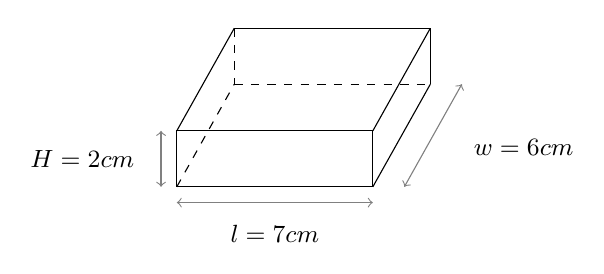
\begin{tikzpicture}[scale=1.0, baseline=(current bounding box.north)]
     \begin{scope}[rotate=0]

    % front face
    \coordinate (A) at (0,0);
    \coordinate (B) at (2.49,0);
    \coordinate (C) at (2.49,0.711);
    \coordinate (D) at (0,0.711);

    % back face skew shift
    \coordinate (E) at ($(A)+(0.73, 1.303)$);
    \coordinate (F) at ($(B)+(0.73, 1.303)$);
    \coordinate (G) at ($(C)+(0.73, 1.303)$);
    \coordinate (H) at ($(D)+(0.73, 1.303)$);

    % draw prism edges
    \draw[] (A)--(B)--(C)--(D)--cycle;
    \draw[dashed] (A)--(E);
    \draw[] (B)--(F);
    \draw[] (C)--(G);
    \draw[] (D)--(H);
    \draw[dashed] (E)--(F);
    \draw[] (F)--(G);
    \draw[] (G)--(H);
    \draw[dashed] (H)--(E);

    % label corners
    % \node[above left] at (A) {A};
    % \node[below right] at (B) {B};
    % \node[above right] at (C) {C};
    % \node[above left] at (D) {D};
    % \node[below left] at (E) {E};
    % \node[below right] at (F) {F};
    % \node[above right] at (G) {G};
    % \node[above left] at (H) {H};

    % dimension lines enabled
    \coordinate (P1offAB) at ($ (A)+(0,-0.2) $);
    \coordinate (P2offAB) at ($ (B)+(0,-0.2) $);
    \draw[<->,gray] (P1offAB)--(P2offAB);
    \node[black, fill=white, fill opacity=1.0, text opacity=1, inner sep=1pt]
        at ($ (P1offAB)!0.5!(P2offAB) + (0,-0.4) $) {\small $l=7 cm$};

    \coordinate (P1offAD) at ($ (A)+(-0.2,0) $);
    \coordinate (P2offAD) at ($ (D)+(-0.2,0) $);
    \draw[<->,gray] (P1offAD)--(P2offAD);
    \node[black, fill=white, fill opacity=1.0, text opacity=1, inner sep=1pt]
        at ($ (P1offAD)!0.5!(P2offAD) + (-1.0,0) $) {\small $H=2 cm$};

    \coordinate (P1offBF) at ($ (B)+(0.4,0) $);
    \coordinate (P2offBF) at ($ (F)+(0.4,0) $);
    \draw[<->,gray] (P1offBF)--(P2offBF);
    \node[black, fill=white, fill opacity=1.0, text opacity=1, inner sep=1pt]
        at ($ (P1offBF)!0.5!(P2offBF) + (1.15,-0.15) $) {\small $w=6 cm$};
    \end{scope}
\end{tikzpicture}
\end{minipage}
\hfill
\begin{minipage}{.5\textwidth}
  \begin{align*}
  \text{Volume} &= lwH \\
  \text{Volume} &= \dotuline{~~~~~} \,\text{cm} \times \dotuline{~~~~~} \,\text{cm} \times \dotuline{~~~~~} \,\text{cm} \\
  \text{Volume} &= \dotuline{~~~~~} \,\text{cm}^3
  \end{align*}
\end{minipage}
\par\vspace{1cm}\begin{minipage}{0.50\textwidth}
  \refstepcounter{minipagecount}
  \noindent{(\theminipagecount)}\quad
  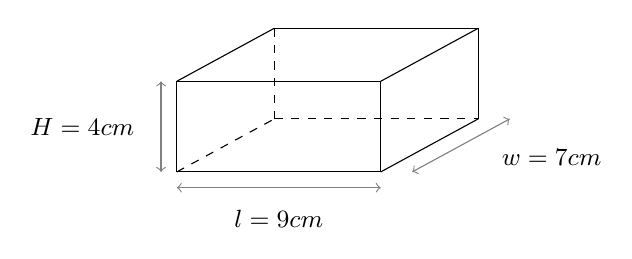
\begin{tikzpicture}[scale=1.0, baseline=(current bounding box.north)]
     \begin{scope}[rotate=0]

    % front face
    \coordinate (A) at (0,0);
    \coordinate (B) at (2.59,0);
    \coordinate (C) at (2.59,1.151);
    \coordinate (D) at (0,1.151);

    % back face skew shift
    \coordinate (E) at ($(A)+(1.239, 0.674)$);
    \coordinate (F) at ($(B)+(1.239, 0.674)$);
    \coordinate (G) at ($(C)+(1.239, 0.674)$);
    \coordinate (H) at ($(D)+(1.239, 0.674)$);

    % draw prism edges
    \draw[] (A)--(B)--(C)--(D)--cycle;
    \draw[dashed] (A)--(E);
    \draw[] (B)--(F);
    \draw[] (C)--(G);
    \draw[] (D)--(H);
    \draw[dashed] (E)--(F);
    \draw[] (F)--(G);
    \draw[] (G)--(H);
    \draw[dashed] (H)--(E);

    % label corners
    % \node[above left] at (A) {A};
    % \node[below right] at (B) {B};
    % \node[above right] at (C) {C};
    % \node[above left] at (D) {D};
    % \node[below left] at (E) {E};
    % \node[below right] at (F) {F};
    % \node[above right] at (G) {G};
    % \node[above left] at (H) {H};

    % dimension lines enabled
    \coordinate (P1offAB) at ($ (A)+(0,-0.2) $);
    \coordinate (P2offAB) at ($ (B)+(0,-0.2) $);
    \draw[<->,gray] (P1offAB)--(P2offAB);
    \node[black, fill=white, fill opacity=1.0, text opacity=1, inner sep=1pt]
        at ($ (P1offAB)!0.5!(P2offAB) + (0,-0.4) $) {\small $l=9 cm$};

    \coordinate (P1offAD) at ($ (A)+(-0.2,0) $);
    \coordinate (P2offAD) at ($ (D)+(-0.2,0) $);
    \draw[<->,gray] (P1offAD)--(P2offAD);
    \node[black, fill=white, fill opacity=1.0, text opacity=1, inner sep=1pt]
        at ($ (P1offAD)!0.5!(P2offAD) + (-1.0,0) $) {\small $H=4 cm$};

    \coordinate (P1offBF) at ($ (B)+(0.4,0) $);
    \coordinate (P2offBF) at ($ (F)+(0.4,0) $);
    \draw[<->,gray] (P1offBF)--(P2offBF);
    \node[black, fill=white, fill opacity=1.0, text opacity=1, inner sep=1pt]
        at ($ (P1offBF)!0.5!(P2offBF) + (1.15,-0.15) $) {\small $w=7 cm$};
    \end{scope}
\end{tikzpicture}
\end{minipage}
\hfill
\begin{minipage}{.5\textwidth}
  \begin{align*}
  \text{Volume} &= lwH \\
  \text{Volume} &= \dotuline{~~~~~} \,\text{cm} \times \dotuline{~~~~~} \,\text{cm} \times \dotuline{~~~~~} \,\text{cm} \\
  \text{Volume} &= \dotuline{~~~~~} \,\text{cm}^3
  \end{align*}
\end{minipage}
\par\vspace{1cm}\begin{minipage}{0.50\textwidth}
  \refstepcounter{minipagecount}
  \noindent{(\theminipagecount)}\quad
  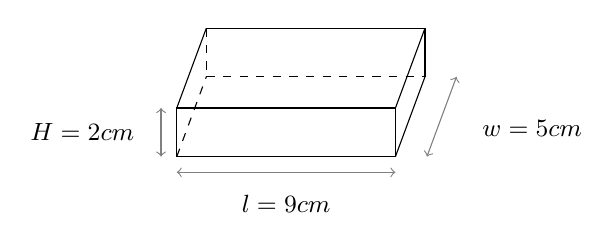
\begin{tikzpicture}[scale=1.0, baseline=(current bounding box.north)]
     \begin{scope}[rotate=0]

    % front face
    \coordinate (Q) at (0,0);
    \coordinate (R) at (2.777,0);
    \coordinate (S) at (2.777,0.617);
    \coordinate (T) at (0,0.617);

    % back face skew shift
    \coordinate (W) at ($(Q)+(0.375, 1.013)$);
    \coordinate (X) at ($(R)+(0.375, 1.013)$);
    \coordinate (Y) at ($(S)+(0.375, 1.013)$);
    \coordinate (Z) at ($(T)+(0.375, 1.013)$);

    % draw prism edges
    \draw[] (Q)--(R)--(S)--(T)--cycle;
    \draw[dashed] (Q)--(W);
    \draw[] (R)--(X);
    \draw[] (S)--(Y);
    \draw[] (T)--(Z);
    \draw[dashed] (W)--(X);
    \draw[] (X)--(Y);
    \draw[] (Y)--(Z);
    \draw[dashed] (Z)--(W);

    % label corners
    % \node[above left] at (Q) {Q};
    % \node[below right] at (R) {R};
    % \node[above right] at (S) {S};
    % \node[above left] at (T) {T};
    % \node[below left] at (W) {W};
    % \node[below right] at (X) {X};
    % \node[above right] at (Y) {Y};
    % \node[above left] at (Z) {Z};

    % dimension lines enabled
    \coordinate (P1offAB) at ($ (Q)+(0,-0.2) $);
    \coordinate (P2offAB) at ($ (R)+(0,-0.2) $);
    \draw[<->,gray] (P1offAB)--(P2offAB);
    \node[black, fill=white, fill opacity=1.0, text opacity=1, inner sep=1pt]
        at ($ (P1offAB)!0.5!(P2offAB) + (0,-0.4) $) {\small $l=9 cm$};

    \coordinate (P1offAD) at ($ (Q)+(-0.2,0) $);
    \coordinate (P2offAD) at ($ (T)+(-0.2,0) $);
    \draw[<->,gray] (P1offAD)--(P2offAD);
    \node[black, fill=white, fill opacity=1.0, text opacity=1, inner sep=1pt]
        at ($ (P1offAD)!0.5!(P2offAD) + (-1.0,0) $) {\small $H=2 cm$};

    \coordinate (P1offBF) at ($ (R)+(0.4,0) $);
    \coordinate (P2offBF) at ($ (X)+(0.4,0) $);
    \draw[<->,gray] (P1offBF)--(P2offBF);
    \node[black, fill=white, fill opacity=1.0, text opacity=1, inner sep=1pt]
        at ($ (P1offBF)!0.5!(P2offBF) + (1.15,-0.15) $) {\small $w=5 cm$};
    \end{scope}
\end{tikzpicture}
\end{minipage}
\hfill
\begin{minipage}{.5\textwidth}
  \begin{align*}
  \text{Volume} &= lwH \\
  \text{Volume} &= \dotuline{~~~~~} \,\text{cm} \times \dotuline{~~~~~} \,\text{cm} \times \dotuline{~~~~~} \,\text{cm} \\
  \text{Volume} &= \dotuline{~~~~~} \,\text{cm}^3
  \end{align*}
\end{minipage}
\par\vspace{1cm}\begin{minipage}{0.50\textwidth}
  \refstepcounter{minipagecount}
  \noindent{(\theminipagecount)}\quad
  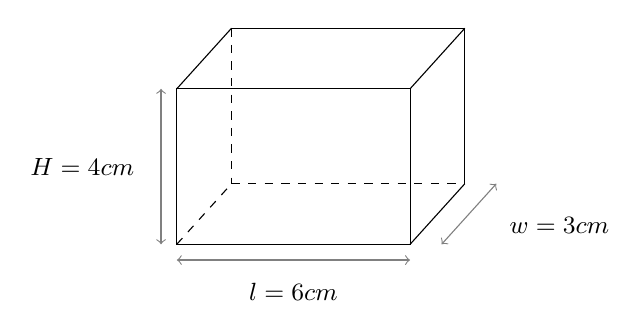
\begin{tikzpicture}[scale=1.0, baseline=(current bounding box.north)]
     \begin{scope}[rotate=0]

    % front face
    \coordinate (Q) at (0,0);
    \coordinate (R) at (2.963,0);
    \coordinate (S) at (2.963,1.975);
    \coordinate (T) at (0,1.975);

    % back face skew shift
    \coordinate (W) at ($(Q)+(0.695, 0.769)$);
    \coordinate (X) at ($(R)+(0.695, 0.769)$);
    \coordinate (Y) at ($(S)+(0.695, 0.769)$);
    \coordinate (Z) at ($(T)+(0.695, 0.769)$);

    % draw prism edges
    \draw[] (Q)--(R)--(S)--(T)--cycle;
    \draw[dashed] (Q)--(W);
    \draw[] (R)--(X);
    \draw[] (S)--(Y);
    \draw[] (T)--(Z);
    \draw[dashed] (W)--(X);
    \draw[] (X)--(Y);
    \draw[] (Y)--(Z);
    \draw[dashed] (Z)--(W);

    % label corners
    % \node[above left] at (Q) {Q};
    % \node[below right] at (R) {R};
    % \node[above right] at (S) {S};
    % \node[above left] at (T) {T};
    % \node[below left] at (W) {W};
    % \node[below right] at (X) {X};
    % \node[above right] at (Y) {Y};
    % \node[above left] at (Z) {Z};

    % dimension lines enabled
    \coordinate (P1offAB) at ($ (Q)+(0,-0.2) $);
    \coordinate (P2offAB) at ($ (R)+(0,-0.2) $);
    \draw[<->,gray] (P1offAB)--(P2offAB);
    \node[black, fill=white, fill opacity=1.0, text opacity=1, inner sep=1pt]
        at ($ (P1offAB)!0.5!(P2offAB) + (0,-0.4) $) {\small $l=6 cm$};

    \coordinate (P1offAD) at ($ (Q)+(-0.2,0) $);
    \coordinate (P2offAD) at ($ (T)+(-0.2,0) $);
    \draw[<->,gray] (P1offAD)--(P2offAD);
    \node[black, fill=white, fill opacity=1.0, text opacity=1, inner sep=1pt]
        at ($ (P1offAD)!0.5!(P2offAD) + (-1.0,0) $) {\small $H=4 cm$};

    \coordinate (P1offBF) at ($ (R)+(0.4,0) $);
    \coordinate (P2offBF) at ($ (X)+(0.4,0) $);
    \draw[<->,gray] (P1offBF)--(P2offBF);
    \node[black, fill=white, fill opacity=1.0, text opacity=1, inner sep=1pt]
        at ($ (P1offBF)!0.5!(P2offBF) + (1.15,-0.15) $) {\small $w=3 cm$};
    \end{scope}
\end{tikzpicture}
\end{minipage}
\hfill
\begin{minipage}{.5\textwidth}
  \begin{align*}
  \text{Volume} &= lwH \\
  \text{Volume} &= \dotuline{~~~~~} \,\text{cm} \times \dotuline{~~~~~} \,\text{cm} \times \dotuline{~~~~~} \,\text{cm} \\
  \text{Volume} &= \dotuline{~~~~~} \,\text{cm}^3
  \end{align*}
\end{minipage}
\par\vspace{1cm}\begin{minipage}{0.50\textwidth}
  \refstepcounter{minipagecount}
  \noindent{(\theminipagecount)}\quad
  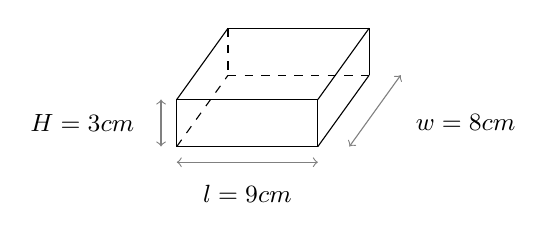
\begin{tikzpicture}[scale=1.0, baseline=(current bounding box.north)]
     \begin{scope}[rotate=0]

    % front face
    \coordinate (Q) at (0,0);
    \coordinate (R) at (1.792,0);
    \coordinate (S) at (1.792,0.597);
    \coordinate (T) at (0,0.597);

    % back face skew shift
    \coordinate (W) at ($(Q)+(0.651, 0.905)$);
    \coordinate (X) at ($(R)+(0.651, 0.905)$);
    \coordinate (Y) at ($(S)+(0.651, 0.905)$);
    \coordinate (Z) at ($(T)+(0.651, 0.905)$);

    % draw prism edges
    \draw[] (Q)--(R)--(S)--(T)--cycle;
    \draw[dashed] (Q)--(W);
    \draw[] (R)--(X);
    \draw[] (S)--(Y);
    \draw[] (T)--(Z);
    \draw[dashed] (W)--(X);
    \draw[] (X)--(Y);
    \draw[] (Y)--(Z);
    \draw[dashed] (Z)--(W);

    % label corners
    % \node[above left] at (Q) {Q};
    % \node[below right] at (R) {R};
    % \node[above right] at (S) {S};
    % \node[above left] at (T) {T};
    % \node[below left] at (W) {W};
    % \node[below right] at (X) {X};
    % \node[above right] at (Y) {Y};
    % \node[above left] at (Z) {Z};

    % dimension lines enabled
    \coordinate (P1offAB) at ($ (Q)+(0,-0.2) $);
    \coordinate (P2offAB) at ($ (R)+(0,-0.2) $);
    \draw[<->,gray] (P1offAB)--(P2offAB);
    \node[black, fill=white, fill opacity=1.0, text opacity=1, inner sep=1pt]
        at ($ (P1offAB)!0.5!(P2offAB) + (0,-0.4) $) {\small $l=9 cm$};

    \coordinate (P1offAD) at ($ (Q)+(-0.2,0) $);
    \coordinate (P2offAD) at ($ (T)+(-0.2,0) $);
    \draw[<->,gray] (P1offAD)--(P2offAD);
    \node[black, fill=white, fill opacity=1.0, text opacity=1, inner sep=1pt]
        at ($ (P1offAD)!0.5!(P2offAD) + (-1.0,0) $) {\small $H=3 cm$};

    \coordinate (P1offBF) at ($ (R)+(0.4,0) $);
    \coordinate (P2offBF) at ($ (X)+(0.4,0) $);
    \draw[<->,gray] (P1offBF)--(P2offBF);
    \node[black, fill=white, fill opacity=1.0, text opacity=1, inner sep=1pt]
        at ($ (P1offBF)!0.5!(P2offBF) + (1.15,-0.15) $) {\small $w=8 cm$};
    \end{scope}
\end{tikzpicture}
\end{minipage}
\hfill
\begin{minipage}{.5\textwidth}
  \begin{align*}
  \text{Volume} &= lwH \\
  \text{Volume} &= \dotuline{~~~~~} \,\text{cm} \times \dotuline{~~~~~} \,\text{cm} \times \dotuline{~~~~~} \,\text{cm} \\
  \text{Volume} &= \dotuline{~~~~~} \,\text{cm}^3
  \end{align*}
\end{minipage}
\par\vspace{1cm}\begin{minipage}{0.50\textwidth}
  \refstepcounter{minipagecount}
  \noindent{(\theminipagecount)}\quad
  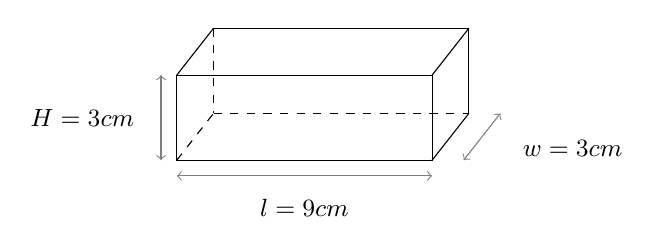
\begin{tikzpicture}[scale=1.0, baseline=(current bounding box.north)]
     \begin{scope}[rotate=0]

    % front face
    \coordinate (Q) at (0,0);
    \coordinate (R) at (3.243,0);
    \coordinate (S) at (3.243,1.081);
    \coordinate (T) at (0,1.081);

    % back face skew shift
    \coordinate (W) at ($(Q)+(0.467, 0.595)$);
    \coordinate (X) at ($(R)+(0.467, 0.595)$);
    \coordinate (Y) at ($(S)+(0.467, 0.595)$);
    \coordinate (Z) at ($(T)+(0.467, 0.595)$);

    % draw prism edges
    \draw[] (Q)--(R)--(S)--(T)--cycle;
    \draw[dashed] (Q)--(W);
    \draw[] (R)--(X);
    \draw[] (S)--(Y);
    \draw[] (T)--(Z);
    \draw[dashed] (W)--(X);
    \draw[] (X)--(Y);
    \draw[] (Y)--(Z);
    \draw[dashed] (Z)--(W);

    % label corners
    % \node[above left] at (Q) {Q};
    % \node[below right] at (R) {R};
    % \node[above right] at (S) {S};
    % \node[above left] at (T) {T};
    % \node[below left] at (W) {W};
    % \node[below right] at (X) {X};
    % \node[above right] at (Y) {Y};
    % \node[above left] at (Z) {Z};

    % dimension lines enabled
    \coordinate (P1offAB) at ($ (Q)+(0,-0.2) $);
    \coordinate (P2offAB) at ($ (R)+(0,-0.2) $);
    \draw[<->,gray] (P1offAB)--(P2offAB);
    \node[black, fill=white, fill opacity=1.0, text opacity=1, inner sep=1pt]
        at ($ (P1offAB)!0.5!(P2offAB) + (0,-0.4) $) {\small $l=9 cm$};

    \coordinate (P1offAD) at ($ (Q)+(-0.2,0) $);
    \coordinate (P2offAD) at ($ (T)+(-0.2,0) $);
    \draw[<->,gray] (P1offAD)--(P2offAD);
    \node[black, fill=white, fill opacity=1.0, text opacity=1, inner sep=1pt]
        at ($ (P1offAD)!0.5!(P2offAD) + (-1.0,0) $) {\small $H=3 cm$};

    \coordinate (P1offBF) at ($ (R)+(0.4,0) $);
    \coordinate (P2offBF) at ($ (X)+(0.4,0) $);
    \draw[<->,gray] (P1offBF)--(P2offBF);
    \node[black, fill=white, fill opacity=1.0, text opacity=1, inner sep=1pt]
        at ($ (P1offBF)!0.5!(P2offBF) + (1.15,-0.15) $) {\small $w=3 cm$};
    \end{scope}
\end{tikzpicture}
\end{minipage}
\hfill
\begin{minipage}{.5\textwidth}
  \begin{align*}
  \text{Volume} &= lwH \\
  \text{Volume} &= \dotuline{~~~~~} \,\text{cm} \times \dotuline{~~~~~} \,\text{cm} \times \dotuline{~~~~~} \,\text{cm} \\
  \text{Volume} &= \dotuline{~~~~~} \,\text{cm}^3
  \end{align*}
\end{minipage}
\par\vspace{1cm}\begin{minipage}{0.50\textwidth}
  \refstepcounter{minipagecount}
  \noindent{(\theminipagecount)}\quad
  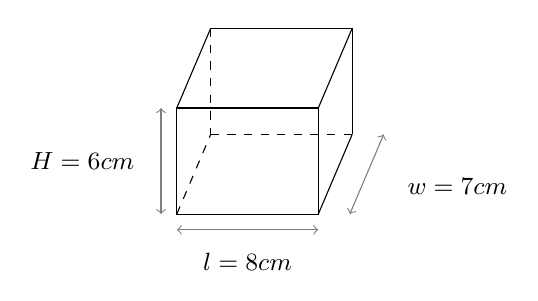
\begin{tikzpicture}[scale=1.0, baseline=(current bounding box.north)]
     \begin{scope}[rotate=0]

    % front face
    \coordinate (Q) at (0,0);
    \coordinate (R) at (1.797,0);
    \coordinate (S) at (1.797,1.348);
    \coordinate (T) at (0,1.348);

    % back face skew shift
    \coordinate (W) at ($(Q)+(0.431, 1.013)$);
    \coordinate (X) at ($(R)+(0.431, 1.013)$);
    \coordinate (Y) at ($(S)+(0.431, 1.013)$);
    \coordinate (Z) at ($(T)+(0.431, 1.013)$);

    % draw prism edges
    \draw[] (Q)--(R)--(S)--(T)--cycle;
    \draw[dashed] (Q)--(W);
    \draw[] (R)--(X);
    \draw[] (S)--(Y);
    \draw[] (T)--(Z);
    \draw[dashed] (W)--(X);
    \draw[] (X)--(Y);
    \draw[] (Y)--(Z);
    \draw[dashed] (Z)--(W);

    % label corners
    % \node[above left] at (Q) {Q};
    % \node[below right] at (R) {R};
    % \node[above right] at (S) {S};
    % \node[above left] at (T) {T};
    % \node[below left] at (W) {W};
    % \node[below right] at (X) {X};
    % \node[above right] at (Y) {Y};
    % \node[above left] at (Z) {Z};

    % dimension lines enabled
    \coordinate (P1offAB) at ($ (Q)+(0,-0.2) $);
    \coordinate (P2offAB) at ($ (R)+(0,-0.2) $);
    \draw[<->,gray] (P1offAB)--(P2offAB);
    \node[black, fill=white, fill opacity=1.0, text opacity=1, inner sep=1pt]
        at ($ (P1offAB)!0.5!(P2offAB) + (0,-0.4) $) {\small $l=8 cm$};

    \coordinate (P1offAD) at ($ (Q)+(-0.2,0) $);
    \coordinate (P2offAD) at ($ (T)+(-0.2,0) $);
    \draw[<->,gray] (P1offAD)--(P2offAD);
    \node[black, fill=white, fill opacity=1.0, text opacity=1, inner sep=1pt]
        at ($ (P1offAD)!0.5!(P2offAD) + (-1.0,0) $) {\small $H=6 cm$};

    \coordinate (P1offBF) at ($ (R)+(0.4,0) $);
    \coordinate (P2offBF) at ($ (X)+(0.4,0) $);
    \draw[<->,gray] (P1offBF)--(P2offBF);
    \node[black, fill=white, fill opacity=1.0, text opacity=1, inner sep=1pt]
        at ($ (P1offBF)!0.5!(P2offBF) + (1.15,-0.15) $) {\small $w=7 cm$};
    \end{scope}
\end{tikzpicture}
\end{minipage}
\hfill
\begin{minipage}{.5\textwidth}
  \begin{align*}
  \text{Volume} &= lwH \\
  \text{Volume} &= \dotuline{~~~~~} \,\text{cm} \times \dotuline{~~~~~} \,\text{cm} \times \dotuline{~~~~~} \,\text{cm} \\
  \text{Volume} &= \dotuline{~~~~~} \,\text{cm}^3
  \end{align*}
\end{minipage}
\par\vspace{1cm}\begin{minipage}{0.50\textwidth}
  \refstepcounter{minipagecount}
  \noindent{(\theminipagecount)}\quad
  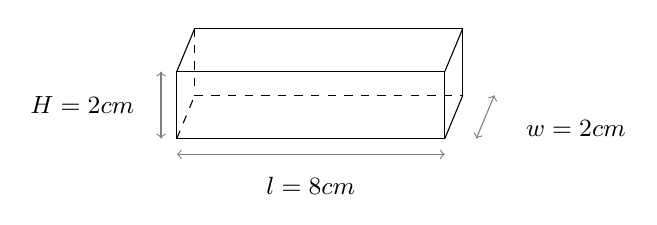
\begin{tikzpicture}[scale=1.0, baseline=(current bounding box.north)]
     \begin{scope}[rotate=0]

    % front face
    \coordinate (E) at (0,0);
    \coordinate (F) at (3.404,0);
    \coordinate (G) at (3.404,0.851);
    \coordinate (H) at (0,0.851);

    % back face skew shift
    \coordinate (K) at ($(E)+(0.229, 0.55)$);
    \coordinate (L) at ($(F)+(0.229, 0.55)$);
    \coordinate (M) at ($(G)+(0.229, 0.55)$);
    \coordinate (N) at ($(H)+(0.229, 0.55)$);

    % draw prism edges
    \draw[] (E)--(F)--(G)--(H)--cycle;
    \draw[dashed] (E)--(K);
    \draw[] (F)--(L);
    \draw[] (G)--(M);
    \draw[] (H)--(N);
    \draw[dashed] (K)--(L);
    \draw[] (L)--(M);
    \draw[] (M)--(N);
    \draw[dashed] (N)--(K);

    % label corners
    % \node[above left] at (E) {E};
    % \node[below right] at (F) {F};
    % \node[above right] at (G) {G};
    % \node[above left] at (H) {H};
    % \node[below left] at (K) {K};
    % \node[below right] at (L) {L};
    % \node[above right] at (M) {M};
    % \node[above left] at (N) {N};

    % dimension lines enabled
    \coordinate (P1offAB) at ($ (E)+(0,-0.2) $);
    \coordinate (P2offAB) at ($ (F)+(0,-0.2) $);
    \draw[<->,gray] (P1offAB)--(P2offAB);
    \node[black, fill=white, fill opacity=1.0, text opacity=1, inner sep=1pt]
        at ($ (P1offAB)!0.5!(P2offAB) + (0,-0.4) $) {\small $l=8 cm$};

    \coordinate (P1offAD) at ($ (E)+(-0.2,0) $);
    \coordinate (P2offAD) at ($ (H)+(-0.2,0) $);
    \draw[<->,gray] (P1offAD)--(P2offAD);
    \node[black, fill=white, fill opacity=1.0, text opacity=1, inner sep=1pt]
        at ($ (P1offAD)!0.5!(P2offAD) + (-1.0,0) $) {\small $H=2 cm$};

    \coordinate (P1offBF) at ($ (F)+(0.4,0) $);
    \coordinate (P2offBF) at ($ (L)+(0.4,0) $);
    \draw[<->,gray] (P1offBF)--(P2offBF);
    \node[black, fill=white, fill opacity=1.0, text opacity=1, inner sep=1pt]
        at ($ (P1offBF)!0.5!(P2offBF) + (1.15,-0.15) $) {\small $w=2 cm$};
    \end{scope}
\end{tikzpicture}
\end{minipage}
\hfill
\begin{minipage}{.5\textwidth}
  \begin{align*}
  \text{Volume} &= lwH \\
  \text{Volume} &= \dotuline{~~~~~} \,\text{cm} \times \dotuline{~~~~~} \,\text{cm} \times \dotuline{~~~~~} \,\text{cm} \\
  \text{Volume} &= \dotuline{~~~~~} \,\text{cm}^3
  \end{align*}
\end{minipage}
\par\vspace{1cm}\begin{minipage}{0.50\textwidth}
  \refstepcounter{minipagecount}
  \noindent{(\theminipagecount)}\quad
  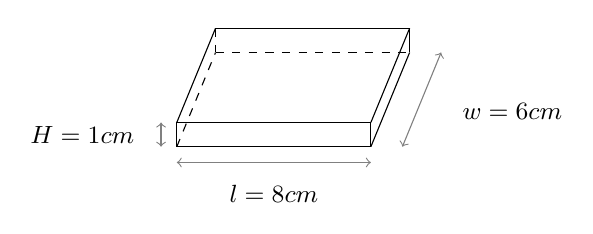
\begin{tikzpicture}[scale=1.0, baseline=(current bounding box.north)]
     \begin{scope}[rotate=0]

    % front face
    \coordinate (Q) at (0,0);
    \coordinate (R) at (2.465,0);
    \coordinate (S) at (2.465,0.308);
    \coordinate (T) at (0,0.308);

    % back face skew shift
    \coordinate (W) at ($(Q)+(0.492, 1.197)$);
    \coordinate (X) at ($(R)+(0.492, 1.197)$);
    \coordinate (Y) at ($(S)+(0.492, 1.197)$);
    \coordinate (Z) at ($(T)+(0.492, 1.197)$);

    % draw prism edges
    \draw[] (Q)--(R)--(S)--(T)--cycle;
    \draw[dashed] (Q)--(W);
    \draw[] (R)--(X);
    \draw[] (S)--(Y);
    \draw[] (T)--(Z);
    \draw[dashed] (W)--(X);
    \draw[] (X)--(Y);
    \draw[] (Y)--(Z);
    \draw[dashed] (Z)--(W);

    % label corners
    % \node[above left] at (Q) {Q};
    % \node[below right] at (R) {R};
    % \node[above right] at (S) {S};
    % \node[above left] at (T) {T};
    % \node[below left] at (W) {W};
    % \node[below right] at (X) {X};
    % \node[above right] at (Y) {Y};
    % \node[above left] at (Z) {Z};

    % dimension lines enabled
    \coordinate (P1offAB) at ($ (Q)+(0,-0.2) $);
    \coordinate (P2offAB) at ($ (R)+(0,-0.2) $);
    \draw[<->,gray] (P1offAB)--(P2offAB);
    \node[black, fill=white, fill opacity=1.0, text opacity=1, inner sep=1pt]
        at ($ (P1offAB)!0.5!(P2offAB) + (0,-0.4) $) {\small $l=8 cm$};

    \coordinate (P1offAD) at ($ (Q)+(-0.2,0) $);
    \coordinate (P2offAD) at ($ (T)+(-0.2,0) $);
    \draw[<->,gray] (P1offAD)--(P2offAD);
    \node[black, fill=white, fill opacity=1.0, text opacity=1, inner sep=1pt]
        at ($ (P1offAD)!0.5!(P2offAD) + (-1.0,0) $) {\small $H=1 cm$};

    \coordinate (P1offBF) at ($ (R)+(0.4,0) $);
    \coordinate (P2offBF) at ($ (X)+(0.4,0) $);
    \draw[<->,gray] (P1offBF)--(P2offBF);
    \node[black, fill=white, fill opacity=1.0, text opacity=1, inner sep=1pt]
        at ($ (P1offBF)!0.5!(P2offBF) + (1.15,-0.15) $) {\small $w=6 cm$};
    \end{scope}
\end{tikzpicture}
\end{minipage}
\hfill
\begin{minipage}{.5\textwidth}
  \begin{align*}
  \text{Volume} &= lwH \\
  \text{Volume} &= \dotuline{~~~~~} \,\text{cm} \times \dotuline{~~~~~} \,\text{cm} \times \dotuline{~~~~~} \,\text{cm} \\
  \text{Volume} &= \dotuline{~~~~~} \,\text{cm}^3
  \end{align*}
\end{minipage}
\par\vspace{1cm}\begin{minipage}{0.50\textwidth}
  \refstepcounter{minipagecount}
  \noindent{(\theminipagecount)}\quad
  \begin{tikzpicture}[scale=1.0, baseline=(current bounding box.north)]
     \begin{scope}[rotate=0]

    % front face
    \coordinate (K) at (0,0);
    \coordinate (L) at (2.14,0);
    \coordinate (M) at (2.14,3.745);
    \coordinate (N) at (0,3.745);

    % back face skew shift
    \coordinate (Q) at ($(K)+(1.039, 0.428)$);
    \coordinate (R) at ($(L)+(1.039, 0.428)$);
    \coordinate (S) at ($(M)+(1.039, 0.428)$);
    \coordinate (T) at ($(N)+(1.039, 0.428)$);

    % draw prism edges
    \draw[] (K)--(L)--(M)--(N)--cycle;
    \draw[dashed] (K)--(Q);
    \draw[] (L)--(R);
    \draw[] (M)--(S);
    \draw[] (N)--(T);
    \draw[dashed] (Q)--(R);
    \draw[] (R)--(S);
    \draw[] (S)--(T);
    \draw[dashed] (T)--(Q);

    % label corners
    % \node[above left] at (K) {K};
    % \node[below right] at (L) {L};
    % \node[above right] at (M) {M};
    % \node[above left] at (N) {N};
    % \node[below left] at (Q) {Q};
    % \node[below right] at (R) {R};
    % \node[above right] at (S) {S};
    % \node[above left] at (T) {T};

    % dimension lines enabled
    \coordinate (P1offAB) at ($ (K)+(0,-0.2) $);
    \coordinate (P2offAB) at ($ (L)+(0,-0.2) $);
    \draw[<->,gray] (P1offAB)--(P2offAB);
    \node[black, fill=white, fill opacity=1.0, text opacity=1, inner sep=1pt]
        at ($ (P1offAB)!0.5!(P2offAB) + (0,-0.4) $) {\small $l=4 cm$};

    \coordinate (P1offAD) at ($ (K)+(-0.2,0) $);
    \coordinate (P2offAD) at ($ (N)+(-0.2,0) $);
    \draw[<->,gray] (P1offAD)--(P2offAD);
    \node[black, fill=white, fill opacity=1.0, text opacity=1, inner sep=1pt]
        at ($ (P1offAD)!0.5!(P2offAD) + (-1.0,0) $) {\small $H=7 cm$};

    \coordinate (P1offBF) at ($ (L)+(0.4,0) $);
    \coordinate (P2offBF) at ($ (R)+(0.4,0) $);
    \draw[<->,gray] (P1offBF)--(P2offBF);
    \node[black, fill=white, fill opacity=1.0, text opacity=1, inner sep=1pt]
        at ($ (P1offBF)!0.5!(P2offBF) + (1.15,-0.15) $) {\small $w=3 cm$};
    \end{scope}
\end{tikzpicture}
\end{minipage}
\hfill
\begin{minipage}{.5\textwidth}
  \begin{align*}
  \text{Volume} &= lwH \\
  \text{Volume} &= \dotuline{~~~~~} \,\text{cm} \times \dotuline{~~~~~} \,\text{cm} \times \dotuline{~~~~~} \,\text{cm} \\
  \text{Volume} &= \dotuline{~~~~~} \,\text{cm}^3
  \end{align*}
\end{minipage}
\par\vspace{1cm}\begin{minipage}{0.50\textwidth}
  \refstepcounter{minipagecount}
  \noindent{(\theminipagecount)}\quad
  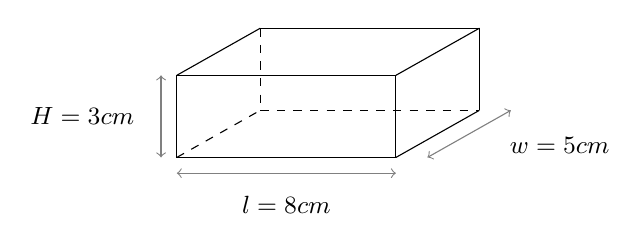
\begin{tikzpicture}[scale=1.0, baseline=(current bounding box.north)]
     \begin{scope}[rotate=0]

    % front face
    \coordinate (Q) at (0,0);
    \coordinate (R) at (2.783,0);
    \coordinate (S) at (2.783,1.043);
    \coordinate (T) at (0,1.043);

    % back face skew shift
    \coordinate (W) at ($(Q)+(1.06, 0.598)$);
    \coordinate (X) at ($(R)+(1.06, 0.598)$);
    \coordinate (Y) at ($(S)+(1.06, 0.598)$);
    \coordinate (Z) at ($(T)+(1.06, 0.598)$);

    % draw prism edges
    \draw[] (Q)--(R)--(S)--(T)--cycle;
    \draw[dashed] (Q)--(W);
    \draw[] (R)--(X);
    \draw[] (S)--(Y);
    \draw[] (T)--(Z);
    \draw[dashed] (W)--(X);
    \draw[] (X)--(Y);
    \draw[] (Y)--(Z);
    \draw[dashed] (Z)--(W);

    % label corners
    % \node[above left] at (Q) {Q};
    % \node[below right] at (R) {R};
    % \node[above right] at (S) {S};
    % \node[above left] at (T) {T};
    % \node[below left] at (W) {W};
    % \node[below right] at (X) {X};
    % \node[above right] at (Y) {Y};
    % \node[above left] at (Z) {Z};

    % dimension lines enabled
    \coordinate (P1offAB) at ($ (Q)+(0,-0.2) $);
    \coordinate (P2offAB) at ($ (R)+(0,-0.2) $);
    \draw[<->,gray] (P1offAB)--(P2offAB);
    \node[black, fill=white, fill opacity=1.0, text opacity=1, inner sep=1pt]
        at ($ (P1offAB)!0.5!(P2offAB) + (0,-0.4) $) {\small $l=8 cm$};

    \coordinate (P1offAD) at ($ (Q)+(-0.2,0) $);
    \coordinate (P2offAD) at ($ (T)+(-0.2,0) $);
    \draw[<->,gray] (P1offAD)--(P2offAD);
    \node[black, fill=white, fill opacity=1.0, text opacity=1, inner sep=1pt]
        at ($ (P1offAD)!0.5!(P2offAD) + (-1.0,0) $) {\small $H=3 cm$};

    \coordinate (P1offBF) at ($ (R)+(0.4,0) $);
    \coordinate (P2offBF) at ($ (X)+(0.4,0) $);
    \draw[<->,gray] (P1offBF)--(P2offBF);
    \node[black, fill=white, fill opacity=1.0, text opacity=1, inner sep=1pt]
        at ($ (P1offBF)!0.5!(P2offBF) + (1.15,-0.15) $) {\small $w=5 cm$};
    \end{scope}
\end{tikzpicture}
\end{minipage}
\hfill
\begin{minipage}{.5\textwidth}
  \begin{align*}
  \text{Volume} &= lwH \\
  \text{Volume} &= \dotuline{~~~~~} \,\text{cm} \times \dotuline{~~~~~} \,\text{cm} \times \dotuline{~~~~~} \,\text{cm} \\
  \text{Volume} &= \dotuline{~~~~~} \,\text{cm}^3
  \end{align*}
\end{minipage}
\par\vspace{1cm}

\end{document}
